\newpage
	\section{D} \label{sec:D}

		\subsection{DEMONSTRABLE}	\index{Demonstrable}	\label{demonstrable}
		Ha  a che vedere con la \underline{\hyperref[technologybaseline]{Technology Baseline}} perchè tratta di essere in grado di convincere che la scelta da noi fatta è buona. In questa circostanza vengono prese le decisioni sulle principali interfacce e configurazioni. \\
		È uno degli stati di progresso del \underline{\hyperref[semat]{SEMAT}} per la \underline{\hyperref[progettazione]{progettazione}}.


		\subsection{DIAGRAMMA DI GANTT} \index{Diagramma di Gantt} \label{gantt}
		Il diagramma mostra la dislocazione temporale delle attività per rappresentarne la durata, la sequenzialità, il parallelismo, e confrontarne le stime con i progressi. \\
		È uno strumento per la \underline{\hyperref[pianificazione]{pianificazione}}.

		\begin{figure}[H]
			\centering
			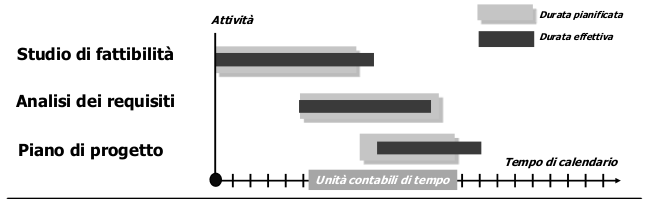
\includegraphics[width=0.7\textwidth]{img/gantt}
			\caption{Esempio di diagramma di Gantt.}
		\end{figure}


		\subsection{DIAGRAMMA DI PERT} \index{Diagramma di PERT} \label{pert}
		Questo tipo di diagramma (\textit{Programme Evaluation and Review Technique}) mostra le dipendenze temporali tra le varie attività al fine di ragionare sulle scadenze di progetto.\\
		È uno strumento per la \underline{\hyperref[pianificazione]{pianificazione}}.

		\begin{figure}[H]
			\centering
			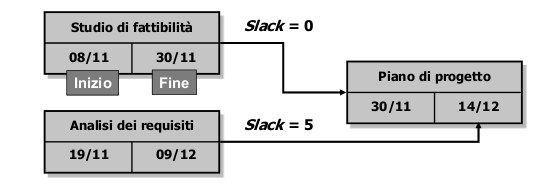
\includegraphics[width=0.7\textwidth]{img/pert}
			\caption{Esempio di diagramma di PERT.}
		\end{figure}

		Si parla qui di \textit{slack time}: periodo di tempo durante il quale un'attività può essere ritardata senza ritardare l'intero progetto di cui fa parte. Si calcola facendo la differenza tra l'ultima data disponibile per compiere l'attività e la prima data disponibile perché venga compiuta. Ha a che vedere con il \underline{\hyperref[camminocritico]{cammino critico}}.

		\subsection{DIMINISHING RETURNS}	\index{Diminishing returns}	\label{diminishingreturn}	%slide 7/34
		\textit{Ritorno in diminuzione} è un certo punto in cui la curva dell'output decresce, ovvero proseguire costa più del beneficio che se ne trae. \\
		È il punto in cui i \underline{\hyperref[test]{test}} non rilevano più errori.

		\subsection{DIVIDE ET IMPERA}	\index{Divide et Impera} \label{divideetimpera}
		Se ho un prodotto fatto di parti riesco ad avere parallelismo nell'implementazione, in modo da andare \textit{n} volte più veloce.

		\subsection{DOCUMENTI}	\index{Documenti}	\label{documenti}
		I documenti adottano una strategia: come mi approccio al problema e come mitigo i rischi. La milestone è definita dalla strategia e applica il \underline{\hyperref[divideetimpera]{divide-et-impera}} perchè divide tutto in problemi più piccoli. Ricordo che la strategia va SEMPRE FATTA ALL'INDIETRO, che vuol dire non pianificare da ora in avanti, ma partire dalla scadenza prefissara e pianificare da quel giorno ad oggi. \\
		Tra i documenti da consegnare nel corso delle revisioni troviamo:
		\begin{itemize}
			\item \underline{\hyperref[piano]{Piano di Progetto}}: quale strategia utilizzare, come nel tempo prepararci ad addomesticare i rischi, ecc
			\item \underline{\hyperref[norme]{Norme di Progetto}}
			\item \underline{\hyperref[pianoqualifica]{Piano di Qualifica}}
			\item \underline{\hyperref[studiofattibilita]{Studio di Fattibilità}}
			\item \underline{\hyperref[analisideirequisiti]{Analisi dei Requisiti}}
			\item \underline{\hyperref[manuali]{Manuali}} tra cui:
			\begin{itemize}
				\item Manuale utente
				\item Manuale sviluppatore
			\end{itemize}
		\end{itemize}

		\subsection{DRIVER}	\index{Driver}	\label{driver}
		È una componente attiva fittizia per pilotare il \underline{\hyperref[test]{test}} e serve per eseguire su un'unità che non ha main.
